\section{Theorie}
\label{sec:Theorie}

% In knapper Form sind die physikalischen Grundlagen des Versuches, des Messverfahrens, sowie sämtliche für die Auswertung erforderlichen Gleichungen darzustellen. (Keine Herleitung)

% (eventuell die Aufgaben)

% Der Versuchsaufbau: Beschreibung des Versuchs und der Funktionsweise (mit Skizze/Bild/Foto)

% Formeln zum Abarbeiten
% -Ladungsträger pro Volumen n
% -Ladungsträger pro Atom z
% -mittlere Flugzeit
% -Driftgeschw.
% -Beweglichkeit
% -Totalgeschw.
% -mittlere freie Weglänge
% -

%%%%%%%%%%

Ein Material wird elektrisch leitend genannt, wenn durch dieses elektrische Ladungen fließen können.
Dabei wird in den meisten Fällen davon ausgegangen, dass der Strom aus negativen Ladungen, also Elektronen besteht.

Da die meisten Metalle freie Elektronen, auch Leitungselektronen genannt, aufweisen, sind diese besonders leitfähig und werden hier näher untersucht.

Die Energienieveaus von Metallatomen sind diskret und können in verschiedene Energiebänder aufgeteilt werden. 
Dabei sind z.B. beim Alkali-Metall die 1s, 2s und 2p Bänder des Na Atoms immer voll mit Elektronen besetzt und diese können weder Energie aufnehmen noch abgeben.
Das 3s Band ist allerdings nur mit einem Elektron gefüllt. 
Daher können Elektronen in diesem Band Energie aufnehmen und bewegen sich bei angelegtem Elektrischen Feld entlang dessen Feldlinien.
So entsteht die elektrische Leitfähigkeit von Metallen. \cite{V311}

Eine Materialkonstante, welche besagt wie gut ein Leiter leitet ist der elektrische Widerstand $R$.
Dieser kann über
\begin{equation}
    R = 2\frac{m_0}{e_0}\frac{1}{n \cdot \bar{\tau}}\frac{L}{Q}
    \label{eq:widerstand}
\end{equation}
bestimmt werden. 
Hier ist $m_0$ die Ruhemasse eines Elektrons, $e_0$ dessen Ladung, $n$ die Ladungsträgerdichte, $\bar{\tau}$ die mittlere Flugzeit der Elektronen, $L$ die Länge des Leiters und $Q$ die Querschnittsfläche des Leiters.

\begin{figure}
    \centering
    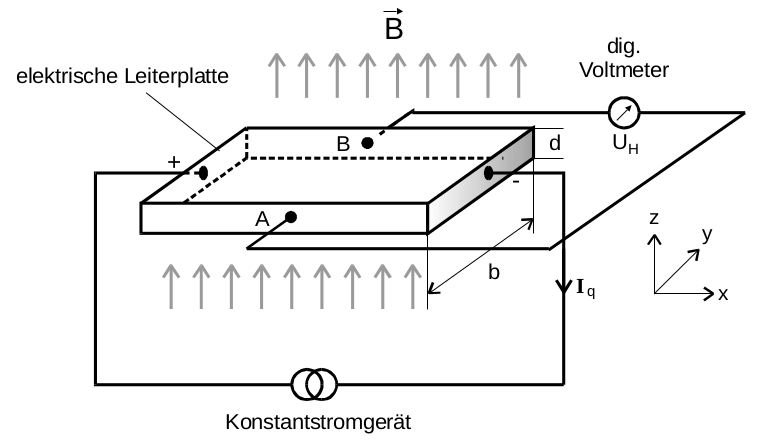
\includegraphics[width=\textwidth]{images/skizze_1.png}
    \caption{Schematischer Versuchsaufbau zur Untersuchung des Hall-Effektes\cite{V311}}
    \label{fig:skizze_1}
\end{figure}

In diesem Versuch werden alle Größen über den Hall-Effekt untersucht.
Wenn wie in \autoref{fig:skizze_1} gezeigt ein Strom durch eine Platte fließt und senkrecht dazu ein Magnetfeld angelegt wird, entsteht eine Spannung zwischen den Punkten A und B.
Diese Spannung wird durch die Lorentz-Kraft verursacht und kann über
\begin{equation}
    U_\text{H} = -\frac{B \cdot I_\text{q}}{n \cdot e_0 \cdot d}
    \label{eq:hallspannung}
\end{equation}
berechnet werden. 
Hier ist $n$ die Anzahl der Ladungsträgerdichte, $e_0$ die Elementarladung, $d$ die Dichte der Platte, $B$ die Magnetfeldstärke und $I_\text{q}$ die Stromstärke des Querstroms.
Diese Spannung wird Hall-Spannung genannt und das Phänomen wird Hall-Effekt genannt.\cite{V311}

